\documentclass[../thesis.tex]{subfiles}
\begin{document}
\section{Test Methodology}
	The experiment evaluates the results of the server by performing benchmark tests. In all the tests, we follow the one-factor-at-a-time experimental design \cite{oaat} to ensure the accuracy and effectiveness of tests.

\subsection{Benchmark Test Methodology}
Benchmark Testing is a type of testing done to give repeatable set of quantifiable result from which present and future software releases for specific functionality can be baselined or compared. It is a process used to compare the performance of software or hardware system also known as SUT (System Under Test). An SUT can be a Web-based application.
\paragraph{}
A benchmark must be repeatable. For instance, with every iteration of load test, if the response times varies too much, system performance be benchmarked. Response time needs to be stable amongst different load conditions.
\paragraph{}
A benchmark must be quantifiable. For example, user experience cannot be quantified in numbers, but time a user spends on a webpage due to good UI can be quantified.

\subsection*{Why benchmark testing is important?}
At business level, benchmark testing can be helpful in determining
\vspace{5mm}
\begin{itemize}
	\item How well a web-based application is performing with respect to the competitors
	\item It ensures that websites complies with standards and best practices
	\item It enables to evaluate third- party service providers prior to making a contracting decision
	\item Allows to figure out the mistakes to be avoided
	\item How different types of customers experience the response time and availability of a site.
\end{itemize}
\subsection{Phases of benchmark testing}
\subsection*{Planning Phase}
\begin{itemize}
	\item Identifying and prioritize standards and requirements
	\item Decide benchmark criteria
	\item Define benchmark test process
\end{itemize}
\subsection*{Analysis Phase}
\begin{itemize}
	\item Identify root cause of error to improve quality
	\item Setting goals for test process
\end{itemize}
\subsection*{Integration Phase}
\begin{itemize}
	\item Share outcomes with concerned person and get approval
	\item Establish functional goals
	\item Define benchmark test process
\end{itemize}
\subsection*{Action Phase}
\begin{itemize}
	\item Develop test plan and documentation
	\item Implement actions specified in previous phases and monitor progress
	\item Run the process continuously
\end{itemize}

\subsection{Testing the web technologies}
According to one-factor-at-a-time experimental design, we make three fundamental tests - "Calculate Value of Fibonacci" and "Fetch data from local DB" and "Fetch data from remote DB". "Calculate Value of Fibonacci" module calculates some value of Fibonacci and evaluates the performance under compute-intensive tests. "Select Operation from local DB" module compares different performance through querying some value of DB in an IO-intensive situation. Under all benchmark tests, we keep requests 100. TABLE 1 summarizes the factors in our experiments.

\begin{table}[H]
	\caption{Benchmark test factors}
	\centering
	\footnotesize
	\label{tab1}
	\begin{tabular}{!{\color{sapphire}\vrule width 1pt}m{0.22\textwidth}!{\color{black}\vrule width 1pt}m{0.22\textwidth}!{\color{black}\vrule width 1pt}m{0.22\textwidth}!{\color{black}\vrule width 1pt}m{0.22\textwidth}!{\color{sapphire}\vrule width 1pt}}
		\arrayrulecolor{sapphire}\hline
		\Centering Requests &
		\Centering 10, 100, 200, 500, 700, 1000 \\
		\hline
		\Centering Benchmark test module & 
		\Centering Calculate fibonacci, SELECT local DB, remote DB \\
		\hline
		\Centering Web technologies tested & 
		\Centering Node, PHP, Python-Django \\
		\hline
		\arrayrulecolor{sapphire}\hline
	\end{tabular}
\end{table} 
\begin{figure}[H]
	\centering
	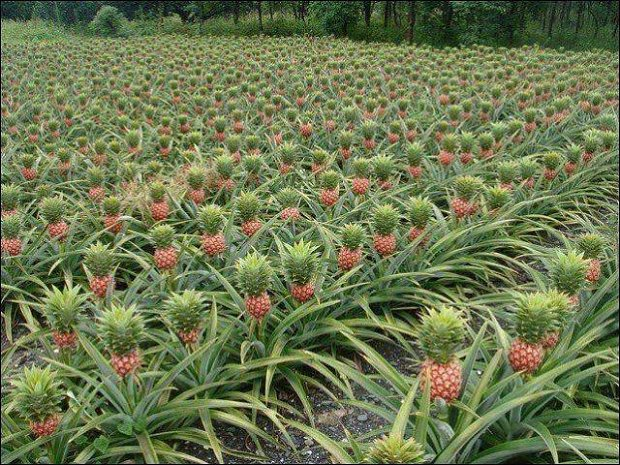
\includegraphics[width=0.65\textwidth]{pole_ananasowe.jpg}
	\captionsetup{justification=raggedleft, font={it, footnotesize}}
	\caption*{\url{http://vader.joemonster.org/upload/qpm/l_13484426e12385bananasplantage.jpg}} 
	\captionsetup{justification=justified, font={up, footnotesize}}
	\caption{Tak wygląda ananasowe pole. Przykład wklejania grafiki rastrowej.}
	\label{rys1}
\end{figure}
\end{document}